\chapter{Design og Implementering}

\section{Hardware}

\subsection{Motorstyring}
\subsubsection{H-bro}
\subsubsection{Detektor}
Denne detektor består af et potentiometer og en ADC, som er en del af “motorstyring” blokken, så ved hjælp af potentiometeret kan man sørge for, at motoren ikke drejer for langt ud til begge sider.  Der kunne være brugt en stepper-motor til at styre det med, men for at få mere hardware med, blev det besluttet, at det var en bedre løsning at gøre det på denne måde.
\begin{figure}[H]
	\centering
	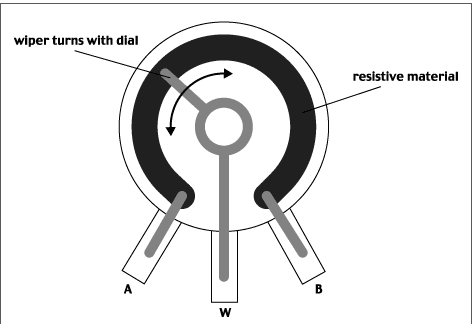
\includegraphics[width=\textwidth]{Afsnit/DesignOgImplementering/images/poten}
	\caption{potentiometer}
	\label{fig:poten}
\end{figure}
\textbf{måske et billede af opstilling i stedet for}\\
Potentiometeret har til formål at skulle holde styr på, at motoren ikke kører længere ud end det hvad det fastsatte krav er. Der er blevet valgt at bruge et Potentiometer som er et linæret et, som vil sige at når man for hver ændring man laver på Potentiometeret, vil der også ske en ændring i output spændingen. Så når den bliver fast gjord til motoren vil man kunne se en ændring i den spænding som kommer ud fra potentiometeret, som bliver sendt ind i ADC’en, som er af typen Sequencing Successive Approximation ADC, som er placeret internt i PSoC’en. Så når output spændingen fra potentiometer bliver aflæst, vil man kunne vide præcise hvor motoren er.  
ADC’en er en sample hold kreds, som vil sige den holder på dataen end til der er fundet en værdi, så der går noget tid i mellem hver værdi, så der er søgeret for at der ikke bliver lavet over samples og der ikke bliver lavet aliasing af det signal som kommer ind i ADC’en. For at finde den værdi som bliver sendt ind i ADC'en, bliver der lavet en skala som bliver halvert alt efter hvor værdien ligger på skalaen, som vist på figur \ref{fig:pot}

\begin{figure}[H]
	\centering
	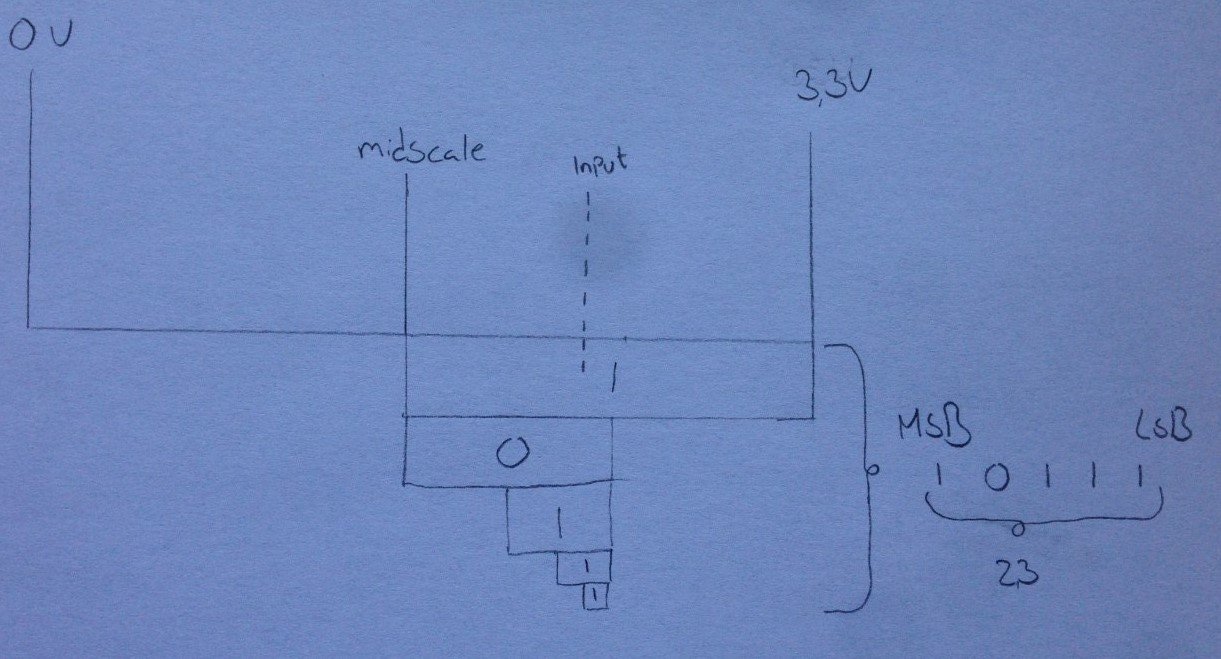
\includegraphics[width=\textwidth]{Afsnit/DesignOgImplementering/images/ADC}
	\caption{ADC opbygning}
	\label{fig:pot}
	\end{figure}

Der er blevet målt med en vinkel måler for at over holde kravene i kravspecifikationen\textbf{\#ref Reference til kravspecikation (ikke funktionelle krav)}. Hvor der blev fundet frem til en min og max hvor motoren må køre i mellem. \\
\\
Min=915 mV\\
\\
Max = 2000mV\\
\\
Disse værdier er aflæst fra PSoC’en, da den har en ref spændingen på 3.3V vil den have lavere værdier end hvad der bliver sendt ud fra Potentiometeret.


\begin{equation}
 \frac {5V} {3.3V}= 1.515
\end{equation}
Der er en forskel på ca. 1.515   mellem potentiometer og ADC. Så ADC er ca. 1,515 mindre end hvad potentiometer sender ud.
\\
For at forstå hvordan ADC’en og potentiometeret fungerer henvises til dokumentationen.

\subsection{Affyringsmekanisme}
Affyringsmekanismen er bygget op af en motor; et motorstyringskredsløb; et detektorkredsløb, der skal detektere, at motoren kun kører en enkelt omgang, når der skydes; og en kanon, som er bygget op af noget mekanik og LEGO. 

\subsubsection{Detektor}
Detektorens formål er at detektere, hvornår motoren har kørt en omgang og derefter slukke den. Princippet i detektoren er, at en fotodiode skal modtage lyssignal fra en LED, hvorefter den skal sende signal om at starte motoren. Når fotodioden ikke længere kan se lyssignalet fra LED'en, skal den sende signal om at slukke motoren igen. Det vil sige, at det er vigtigt, at det kun er lyset fra LED'en fotodioden kan se. Dette sikres ved at sætte LED'en til at lyse med en frekvens på 10 kHz og lave et båndpasfilter, som kun lader disse frekvenser opfanges i fotodioden. 

Dette båndpasfilter er opbygget af et højpasfilter og et lavpasfilter. Til at sende signal om, at motoren skal køre bruges, at når fotodioden kan se LED'en skal den sende et højt signal ud. Her bruges PSoC'ens operationsforstærker. For at gøre dette signal til et pænt firkantsignal, blev der lavet en envelopedetector, som er opbygget af en diode, en modstand og en kondensator. 

Det signal, som kom fra PSoC'en var dog for lavt til at kunne blive opfattet som et højt signal. Derfor 

\subsubsection{Motorstyring}
Til at styre affyringsmekanismens motor er der bygget et kredsløb med en MOSFET som primære komponent. MOSFET'en skal sørge for, at motoren kun kører, når der bliver sendt PWM-signal ind i den. 


\subsubsection{Kanon}
Selve kanonen i systemet er bygget op af to træplader og LEGO. Den ene træplade skal kunne dreje fra side til side, således at det er muligt at sigte i den horisontale retning. Den vertikale retning er bygget af LEGO, ligesom selve kanonen også er bygget i LEGO. 

\section{Software}

\subsection{SPI - Devkit8000}
Candydriveren sørger for SPI-kommunikationen fra Devkit8000 til PSoC0. Driveren er skrevet i c, hvilket er typisk for drivere til linuxplatforme.\\
SPI-kommunikationen er implementeret med SPI bus nummer 1, SPI chip-select 0 og en hastighed på 1 MHz (et godt stykke under max på 20 MHz for en sikkerhedsskyld). Desuden starter clocken højt og data ændres på falling edge og aflæses på rising edge. Dermed bliver SPI Clock Mode 3. Derudover sendes der 8 bit pr transmission, hvilket passer med SPI-protokollen for projektet.\\
For at kunne anvende driveren, når SPI er tilsluttet, er der oprettet et hotplugmodul, som fortæller kernen, at der er et SPI device, som matcher driveren. Det kan SPI-forbindelsen ikke selv gøre, som usb fx kan. Selve driveren er i candygun.c opbygget som en char driver. For at holde forskellige funktionaliteter adskilt er alle funktioner, der har med SPI at gøre, implementeret i filen candygun-spi-c. Så når der fx skal requestes en SPI ressource i init-funktionen i candygun.c, så anvender driveren en funktion fra candygun-spi.c til det. I probe-funktionen sættes bits\textunderscore per\textunderscore word til 8, da vi sender otte bit som nævnt tidligere. I exit-funktionen anvender candygun.c igen en funktion fra candygun-spi.c - denne gang til at frigive SPI ressourcen. I write-metoden gives der data med fra brugeren. I dette tilfælde udgøres brugeren af Interface driveren og dataet er en 8 bit kommando fra SPI-protokollen. Dog er dataet fra brugeren i første omgang læst ind som en charstreng. I write-metoden bliver det så lavet om til en int.  For at overføre dataet på en sikker måde anvendes funktionen copy\textunderscore from\textunderscore user() til at overføre data fra brugeren. Write-funktionen fra candygun.c anvender derefter en write-funktion fra candygun-spi.c, hvor den sender brugerinputtet med. I den spi-relaterede write-funktion bliver bruger inputtet lagt i transfer bufferen og der NULL bliver lagt i receive bufferen, og med spi\textunderscore sync-funktionen bliver det sendt.\\ 
Ofte ville der en spi read-funktion først indeholde en write-del, som fortalte SPI-slaven, hvad der skulle læses over i bufferen. Det ville typisk efterfølges af et delay og så en read-del. Men i dette projekt skal der ofte afventes et brugerinput, som ikke kan styres af et fast delay, og der skal generelt sendes en aktiv kommando før der læses. Derfor er det besluttet at read-funktionen kun indeholder en read-del i transmissionen. Dermed skal write-funktionen altid aktivt anvendes inden der læses, da PSoC0 ellers ikke ved, hvad der skal gøres/lægges i bufferen.\\
Når funktionen har modtaget resultatet fra transmissionen returneres det til brugeren med funktionen copy\textunderscore to\textunderscore user(), som igen sørger for at overførslen af data foregår på en sikker måde.   


\subsection{Interface Driver}
Interface driveren fungerer som bindeled mellem brugergrænsefladen og candydriveren på Devkit8000. Den indeholder tre funktioner. Funktionerne anvendes i use case 2 til at teste kommunikationsforbindelserne i resten af systemet. Interface driveren er designet og implementeret i C++ og gør brug af klasserelationen arv. Et klassediagram for interface driveren se på figur  \ref{fig:idriveruc2}.\\

\begin{figure}[H]
	\centering
	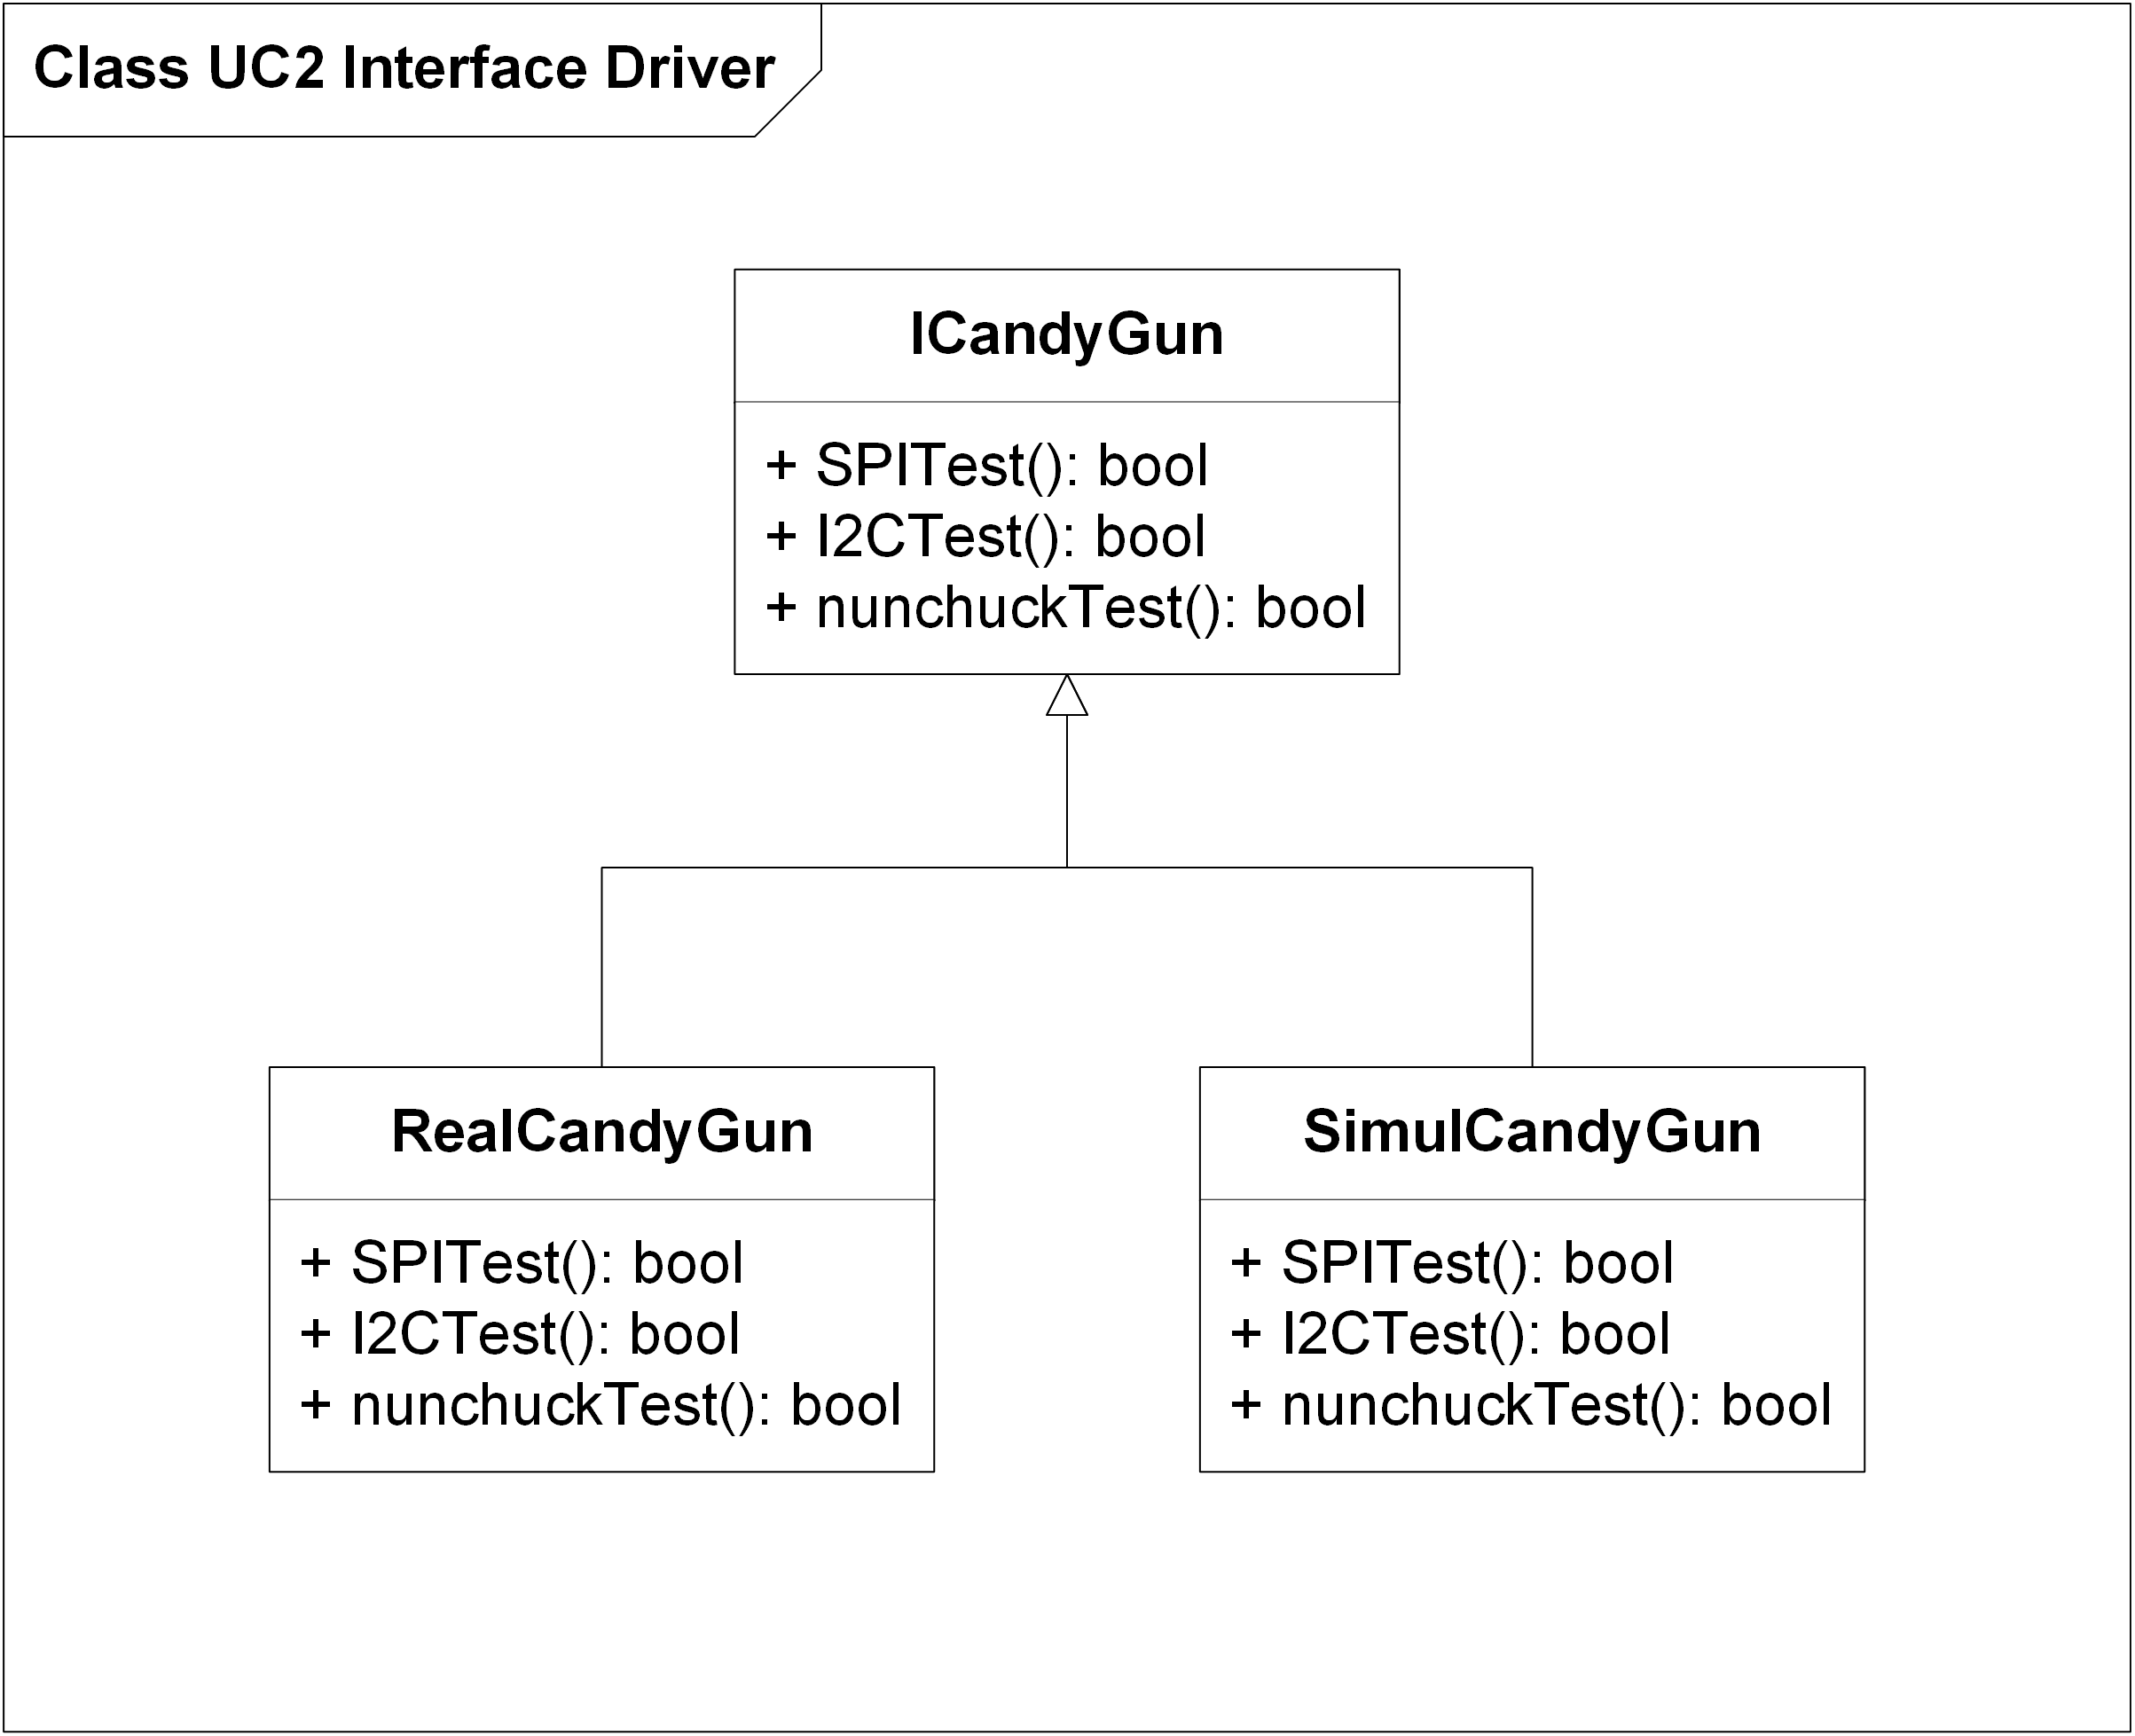
\includegraphics[width=\textwidth]{Afsnit/DesignOgImplementering/images/IdriverKlasseDiagram}
	\caption{Interface driver for UC2}
	\label{fig:idriveruc2}
\end{figure}

Basisklassen er ICandyGun. Det er en abstrakt klasse, da den udelukkende indeholder virtuelle metoder. Derudover er der to afledte klasser; SimulCandyGun og RealCandyGun. SimulCandyGun implementerer metoderne til at simulere respons fra Candydriveren. Dermed kan brugergrænsefladen testes uafhængigt af de resterende dele af systemet. Simuleringen er implementeret med \textit{srand()}-funktionen fra \textit{cstdlib}-biblioteket, som returnerer et tilfældigt tal, som her bliver mellem 0 og 1. I RealCandyGun-klassen er metoderne implementeret efter den reelle SPI-protokol og med de nødvendige funktioner til at skrive til et kernemodul. Fx open(), close(), read () og write(). Da interface driveren er implementeret med arv, skal der ikke foretages betydelige ændringer i brugergrænsefladen, når der skiftes mellem simuleringsklassen og den rigtige version. Dermed opnås lav kobling. \\
De tre funktioner som Interface driveren indeholder i forbindelse med use case 2 (test use casen) er: SPITest(), I2CTest(), NunchuckTest(). Hver af de tre funktioner anvendes til at starte en test af de forskellige kommunikationsforbindelser: SPI, I2C og brugerinputet fra nunchucken. Alle funktionerne returnerer en bool, som enten er true eller false, alt efter om testen var succesful eller ej. Når der skal startes en test, åbner den pågældende funktion filen \textit{dev/candygun} og skriver SPI-kommandoen for \textit{start test} til filen. Derefter venter funktionen ét sekund og læser så svaret fra filen. Da der i nunchucktesten ventes på et brugerinput, og brugeren skal have lidt tid til at trykke på nunchuck-knappen, er der oprettet en while-løkke, som tjekker flere gange om testen returnerer true. Hvis testen ikke returnerer true ved første check, venter funktionen atter et sekund og tjekker igen. Det gør den op til 15 gange og melder derefter om fejl, hvis ikke den returnerer true inden.\\
Brugergrænsefladen anvender interface driveren ved at inkludere headerfilerne og oprette en ICandyGun pointer, der peger på en instans af én af de to afledte klasser. Ved at pakke kommunikationen  til kernemodulet for candydriveren væk i funktioner kan brugergrænsefladen anvende funktionerne uden at kende til SPI-protokollen. Det sikrer igen lav kobling, og i tilfælde hvor det kunne ønskes, at SPI-kommunikationen kan erstattes af en anden kommunikationsform, kan det gøres uden, at der skal foretages ændringer i brugergrænsefladen.\\
 
\subsection{Brugergrænseflade}
Selve Usecase 2 styres via brugergrænsfladen fra Devkit8000.
Dette afsnit beskriver brugergrænsefladens design.

\begin{figure}[H]
	\centering
	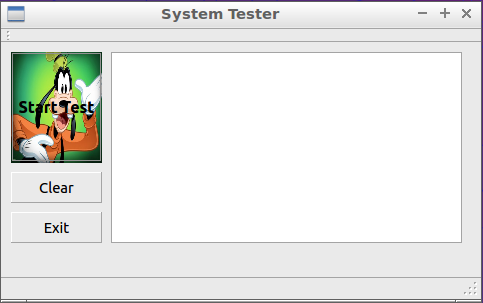
\includegraphics[width=\textwidth]{Afsnit/DesignOgImplementering/images/GUIPic}
	\caption{Brugergrænseflade for usecase 2}
	\label{fig:GUIPic}
\end{figure}

Brugergrænsefladen er lavet med det indbyggede design framework i QT Creator 5.
QT frameworket opretter "hovedvinduet" i brugergrænsefladen som en klasse. Knapperne tilføjes som private slots i klassen
hvilket gør dem i stand til interagere i brugergrænsefladen. Når en knap er assignet til et slot i klassen, og der trykkes på den pågældende knap, bliver det assignede signal broadcastet
og slot-funktionen bliver kørt. Alle tre knapper i brugergrænsefladen er assignet signal-typen "clicked()".

\begin{figure}[H]
	\centering
	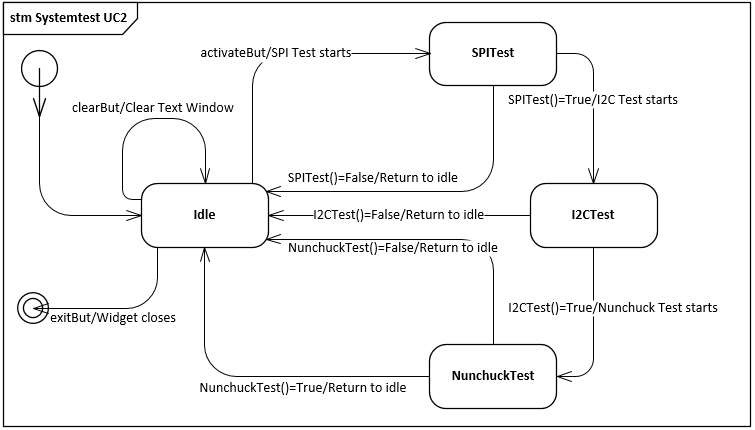
\includegraphics[width=1.2\textwidth]{Afsnit/DesignOgImplementering/images/StateMachineUC2}
	\caption{State machine for brugergrænsefladen for usecase 2}
	\label{fig:StateMachineUC2}
\end{figure}

Brugergrænsefladen for UC2 er en simpel test-konsol. Den består af 3 knapper og et tekstvindue. Brugergrænsefladen interfacer med SPI-protokollen, gennem vores interface driver. Den første knap, Start test, initierer UC2. Efterhånden som testen løbes igennem kaldes test funktionerne, og ved hjælp af if-conditions, bliver der tjekket på retur-værdierne fra interface-funktionerne. Hvis retur-værdien er true, skrives der en "--test successful" besked i tekstvinduet. og widgeten kører videre. Hvis retur-værdien er false, skrives der en "--test unsuccessful" i tekstvinduet og widgeten returnerer til idle tilstand. Når alle test er successful, skrives "System test successful, system is ready for use" til tekstvinduet, og widgeten returnerer til idle tilstand. Den anden knap, Clear, clearer tekstvinduet til blank tilstand. Den tredje knap, Exit, lukker widgeten.

\subsection{Nunchuck}
Til styring af kanonen bruges en Wii-nunchuck. Følgende afsnit beskriver PSoC0's håndtering af data fra Wii-nunchuck.

\subsubsection{Afkodning af Wii-Nunchuck Data Bytes}
Aflæste bytes fra Wii-Nunchuck - indeholdende tilstanden af knapperne og det analoge stick - er kodet når de oprindeligt modtages via I2C bussen. Disse bytes skal altså afkodes før deres værdier er brugbare. Afkodningen af hver byte sker ved brug af følgende formel:

\textit{AfkodetByte = (AflæstByte XOR 0x17) + 0x17}

Fra formlen kan det ses at den aflæste byte skal \textit{XOR}'s (Exclusive Or) med værdien 0x17, hvorefter dette resultat skal adderes med værdien 0x17.

\subsubsection{Kalibrering af Wii-Nunchuck Analog Stick}
De afkodede bytes for Wii-Nunchuck's analoge stick har definerede standardværdier for dets forskellige fysiske positioner. Disse værdier findes i tabel \ref{tabel:WiiNunchuckStickPositioner}

\begin{table}[H]
	\centering
	\begin{tabular}{|l|l|}
		\hline
		X-akse helt til venstre & 0x1E \\ \hline
		X-akse helt til højre   & 0xE1 \\ \hline
		X-akse centreret        & 0x7E \\ \hline
		Y-akse centreret        & 0x7B \\ \hline
		Y-akse helt frem        & 0x1D \\ \hline
		Y-akse helt tilbage     & 0xDF \\ \hline
	\end{tabular}
	\caption{Standardværdier for fysiske positioner af Wii-Nunchuck's analoge stick}
	\label{tabel:WiiNunchuckStickPositioner}
\end{table}

I praksis skal de afkodede værdier for det analoge stick kalibreres, da slør pga. brug gør at de ideale værdier ikke rammes. 

I projektet er de afkodede værdier for det analoge stick kalibreret med værdien -15 (0x0F i hexadecimal), altså ser den endelige formel for afkodning samt kalibrering således ud:

\textit{AfkodetByte = (AflæstByte XOR 0x17) + 0x17 - 0x0F}

\subsection{PSoC Software}
De følgende klassediagrammer på figur \ref{figure:klassediagramPSoC0} og \ref{figure:klassediagramPSoC1} giver et overblik over hvilke klasser der bliver gjort brug af på PSoC0 og PSoC1. De efterfølgende afsnit vil beskrive klasserne og deres funktioner.

\begin{figure}[H]
	\centering
	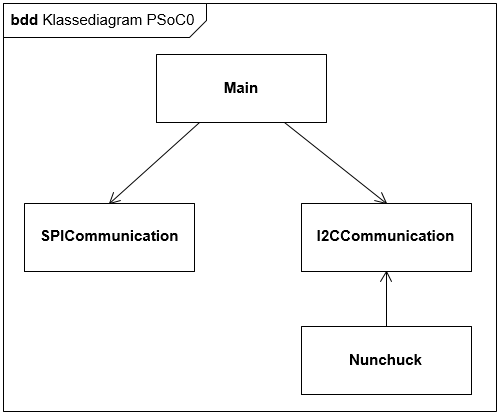
\includegraphics[width=.7\textwidth]{DesignOgImplementering/images/PSoC0KlassediagramOversigt}
	\caption{Klassediagram oversigt for PSoC0}
	\label{figure:klassediagramPSoC0}
\end{figure}

\begin{figure}[H]
	\centering
	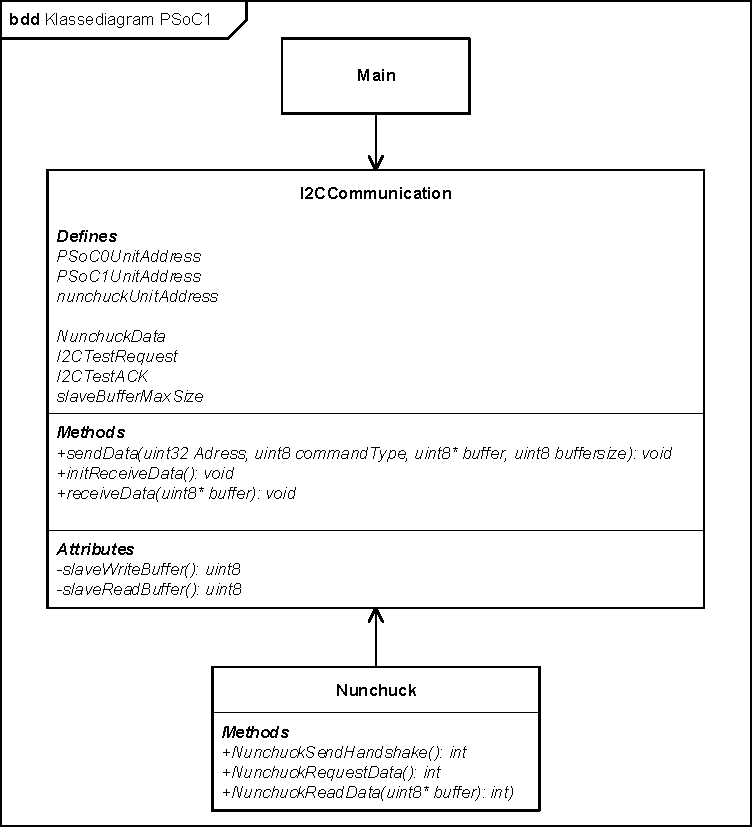
\includegraphics[width=.7\textwidth]{DesignOgImplementering/images/PSoC1KlassediagramOversigt}
	\caption{Klassediagram oversigt for PSoC1}
	\label{figure:klassediagramPSoC1}
\end{figure}

\subsection{I2CCommunication}
I dette afsnit vil softwaren der omhandler I2C-kommunikation blive beskrevet. Dette inkluderer et klassediagram, samt en klassebeskrivelse.
\subsubsection{Klassediagram}
På figur \ref{figure:klassediagramI2CCommunication} ses klassediagrammet for I2CCommunication. 
\begin{figure}[H]
	\centering
	%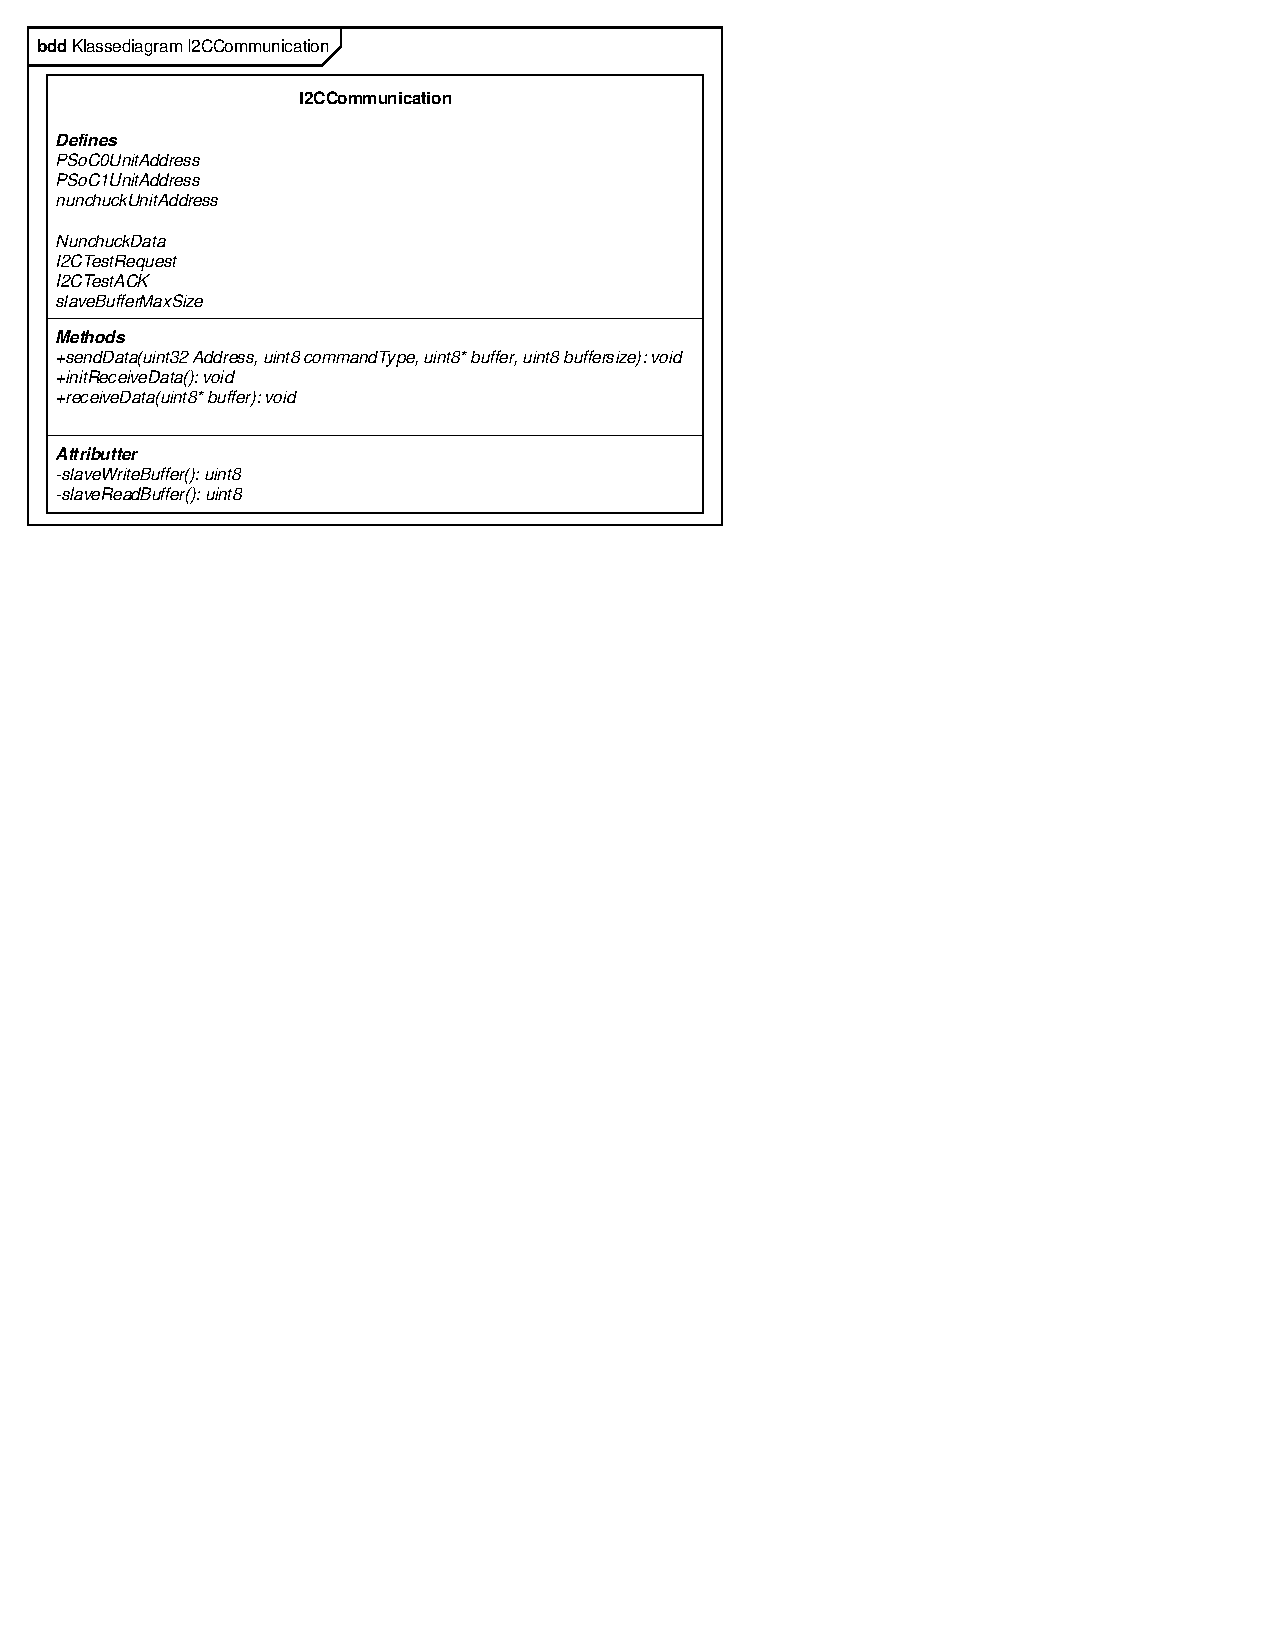
\includegraphics[width=0.9\textwidth, trim={0 19cm 9cm 0},clip]{DesignOgImplementering/images/I2CCommunication.pdf}
	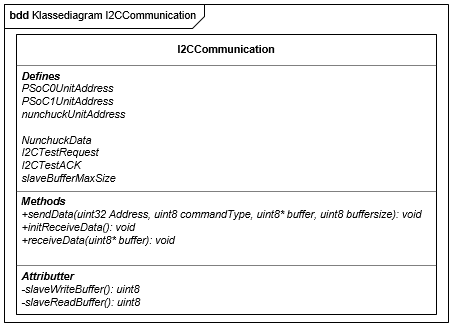
\includegraphics[]{DesignOgImplementering/images/I2CCommunication}
	%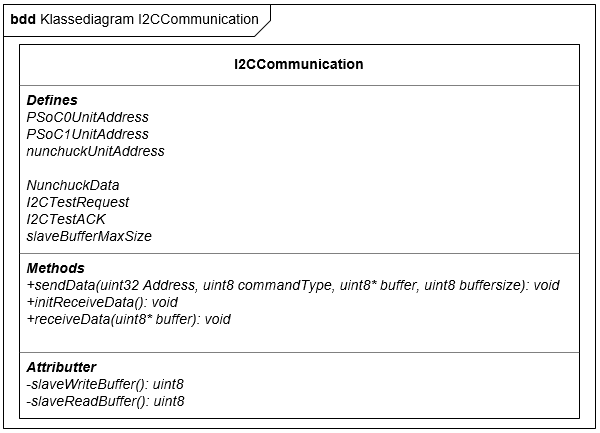
\includegraphics[width =0.9\textwidth]{DesignOgImplementering/images/I2CCommunication2}
	\caption{Klassediagram for I2CCommunication klassen}
	\label{figure:klassediagramI2CCommunication}
\end{figure}

\subsection{Nunchuck}
I dette afsnit vil softwaren der specifikt omhandler kommunikationen mellem PSoC0 og Nunchucken blive beskrevet. Dette gøres vha. et klassediagram og klassebeskrivelser.

\subsubsection{Klassediagram}
På figur \ref{figure:NunchuckKlassediagram} ses klassediagrammet for Nunchuck klassen.

\begin{figure}[H]
	\centering
	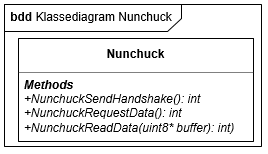
\includegraphics[]{DesignOgImplementering/images/nunchuck}
	\caption{Klassediagram for klassen Nunchuck}
	\label{figure:NunchuckKlassediagram}
\end{figure}

\subsection{SPI - PSoC}
I dette afsnit vil softwaren der specifikt omhandler SPI-kommunikationen mellem PSoC0 og DevKit8000 blive beskrevet. Dette gøres vha. et klassediagram og klassebeskrivelser

\subsubsection{Klassediagram}
På figur \ref{figure:KlassediagramSPICommunication} ses klassediagrammet over SPICommunication klassen.

\begin{figure}[H]
	\centering
	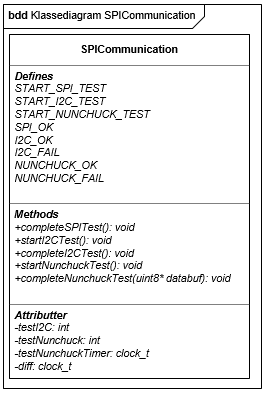
\includegraphics[]{DesignOgImplementering/images/SPICommunication}
	\caption{Klassediagram over klassen SPICommunication}
	\label{figure:KlassediagramSPICommunication}
\end{figure}